%%%%%%%%%%%%%%%%%%%%%%%%%%%%%%%%%%%%%%%%%%%%%%%%%%%%%%%%%%%%%%%%%%%%%%
% Problem statement
\begin{statement}[
  timelimit=1 s,
  memorylimit=512 MiB,
]{H: Herojski Histogram}

Svakom cijelom broju $j$ između $1$ i $n$ pridružen je broj $h_j$. Te brojeve
ćemo prikazivati histogramom. Histogram crtamo tako da za svaki broj $j$
nacrtamo stupac širine $1$ i visine $h_j$ te sve takve stupce uredno posložimo
na $x$-os slijeva nadesno počevši od ishodišta.

\setlength{\belowcaptionskip}{-10pt}
\begin{figure}[H]
\centering
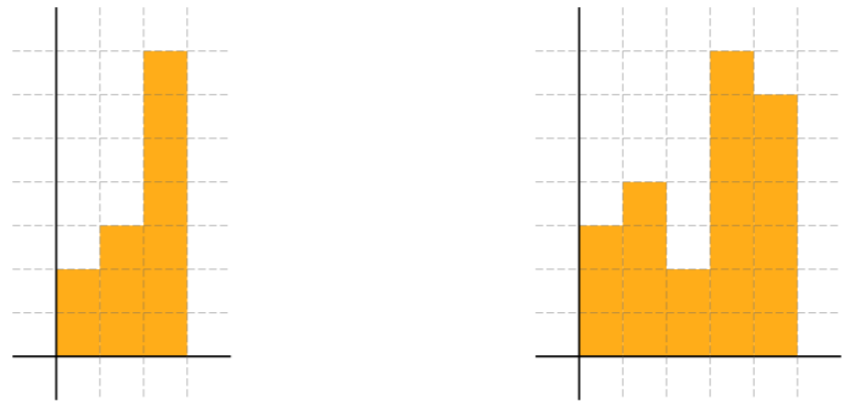
\includegraphics[width=0.5\textwidth]{pic/histogram.png}
\caption{Primjeri histograma koji odgovaraju probnim primjerima.}
\end{figure}

Milan ima jedan takav histogram i na njega želi zalijepiti poster pravokutnog
oblika na kojemu je prikazan njegov najveći heroj -- gospodin Malnar.

Za pravokutnik kažemo da je pravilno pozicioniran unutar histograma ako mu
vrhovi imaju cjelobrojne koordinate, stranice su mu paralelne s koordinatnim
osima te je unutrašnjost tog pravokutnika u potpunosti prekrivena histogramom.

Odredite za svaki broj $j$ između $1$ i $n$ iznos najveće površine pravokutnika
koji se može pravilno pozicionirati unutar prvih $j$ stupaca histograma.

%%%%%%%%%%%%%%%%%%%%%%%%%%%%%%%%%%%%%%%%%%%%%%%%%%%%%%%%%%%%%%%%%%%%%%
% Input
\subsection*{Ulazni podaci}
U prvom je retku prirodni broj $n$ $(1 \le n \le 2 \cdot 10^5)$,  broj stupaca u
histogramu.

U sljedećem se retku nalazi $n$ prirodnih brojeva $h_1$, $h_2$, \dots, $h_n$
$(1 \le h_i \le 10^7)$, visine stupaca u histogramu.


%%%%%%%%%%%%%%%%%%%%%%%%%%%%%%%%%%%%%%%%%%%%%%%%%%%%%%%%%%%%%%%%%%%%%%
% Output
\subsection*{Izlazni podaci}
U jedini redak ispišite $n$ brojeva, $j$-ti od tih brojeva predstavlja iznos
najveće površine pravokutnika koji se može pravilno pozicionirati unutar
prvih $j$ stupaca histograma.

%%%%%%%%%%%%%%%%%%%%%%%%%%%%%%%%%%%%%%%%%%%%%%%%%%%%%%%%%%%%%%%%%%%%%%
% Examples
\subsection*{Probni primjeri}
\begin{tabularx}{\textwidth}{X'X}
  \textbf{ulaz}
  \linespread{1}{\verbatiminput{test/H.dummy.in.1}}
  \textbf{izlaz}
  \linespread{1}{\verbatiminput{test/H.dummy.out.1}} &
  \textbf{ulaz}
  \linespread{1}{\verbatiminput{test/H.dummy.in.2}}
  \textbf{izlaz}
  \linespread{1}{\verbatiminput{test/H.dummy.out.2}}
\end{tabularx}

%%%%%%%%%%%%%%%%%%%%%%%%%%%%%%%%%%%%%%%%%%%%%%%%%%%%%%%%%%%%%%%%%%%%%%
% We're done
\end{statement}

%%% Local Variables:
%%% mode: latex
%%% mode: flyspell
%%% ispell-local-dictionary: "croatian"
%%% TeX-master: "../studentsko2018.tex"
%%% End:
